%!TEX root = ../report.tex

\section{Design Pattern}


\subsection{Structural Pattern}

\subsubsection{Adapter Pattern/Wrapper}
Connects incompatible components to for example
\begin{itemize}
  \item Reuse existing components
  \item Convert an interface to another interface (maybe needed by an API call)
\end{itemize}

Structure:\\
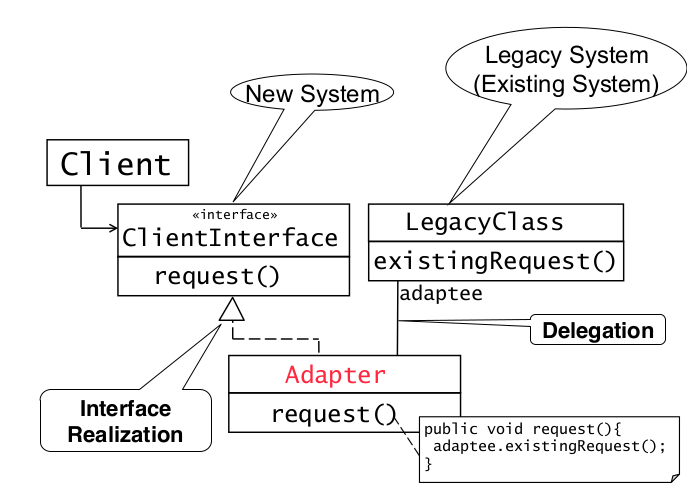
\includegraphics[width=\linewidth]{design_pattern/adapter.png}


\subsubsection{Bridge Pattern}
Allows to delay the assignment of an implementation of an interface from compile to run time.\\
Structure:\\
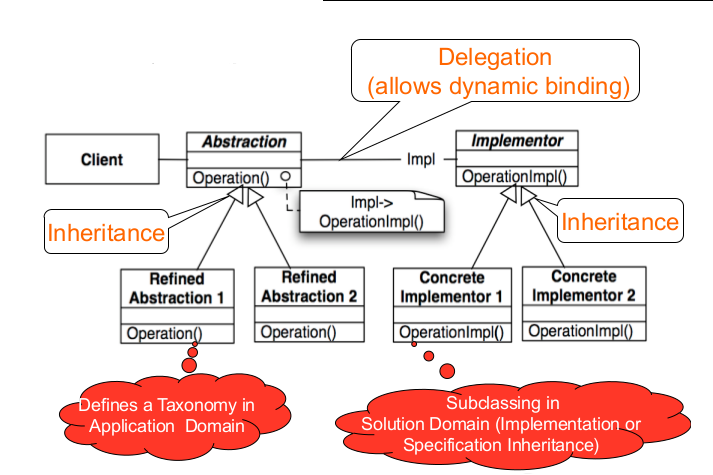
\includegraphics[width=\linewidth]{design_pattern/bridge.png}
The \textbf{degenerated bridge pattern} is the same as the bridge pattern without the taxonomy in the application domain.

\subsubsection{Proxy Pattern/Caching}
The proxy pattern allows to defer object creation and object initialization to the time you need the object (Remote Proxy (Caching), Substitute (Virtual Proxy), Protection Proxy (Access control/Firewall)).\\
Structure:\\
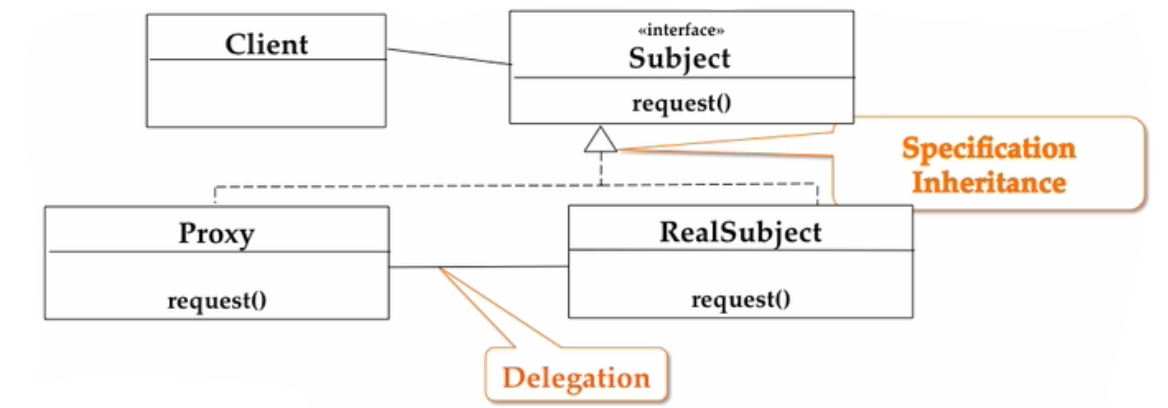
\includegraphics[width=\linewidth]{design_pattern/proxy.png}
The client never calls request() in RealSubject, instead it always calls the method in Proxy which might delegate it to the RealSubject.

\subsubsection{Composite Pattern}
The composite pattern models tree structures that represent part-whole hierarchies with arbitrary depth and width.
It lets the client treat individual objects and groups uniformly. \\
Structure:\\
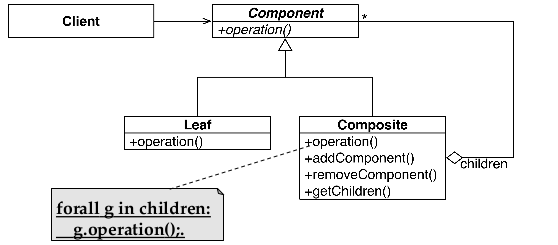
\includegraphics[width=\linewidth]{design_pattern/composite.png}


\subsection{Behavioral Pattern}

\subsubsection{Strategy Pattern}
Suited for situations where different algorithms are available for a problem (e.g. sorting).\\
Structure:\\
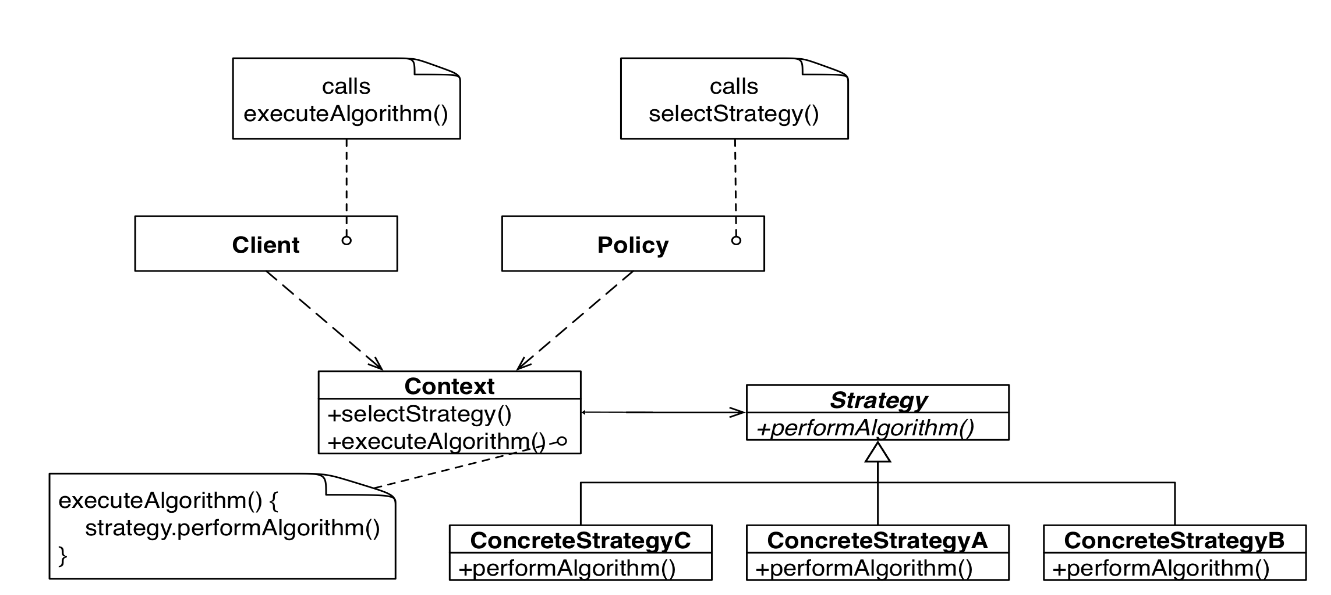
\includegraphics[width=\linewidth]{design_pattern/strategy.png}
A strategy is chosen on \textbf{runtime} by the Policy class before the client calls executeAlgorithm.

\subsubsection{State Pattern}
Dependent on the current state of a system, an action should do different things (e.g. TCP open, close).
The state pattern avoids many if else statements and is flexible to add more cases/states.\\
Structure:\\
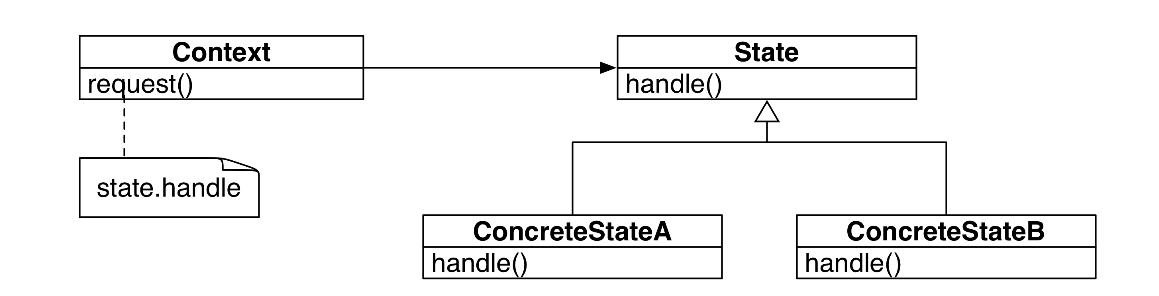
\includegraphics[width=\linewidth]{design_pattern/state.png}
Problem: Where are state transactions handled? (in the exercise of the lecture in the states)

\subsubsection{Observer Pattern}
The observer pattern handles changes in a publisher class and notifies all subscribers about that change (e.g. the user interface) to maintain consistency.
There are three variants for maintaining consistency:
\begin{itemize}
  \item \textbf{Push Notification:} Every time a state changes, all subscribers are notified
  \item \textbf{Push-Update Notification:} The publisher also sends the state that has changed
  \item \textbf{Pull Notification:} A subscriber inquires about the state of the publisher
\end{itemize}
Structure:\\
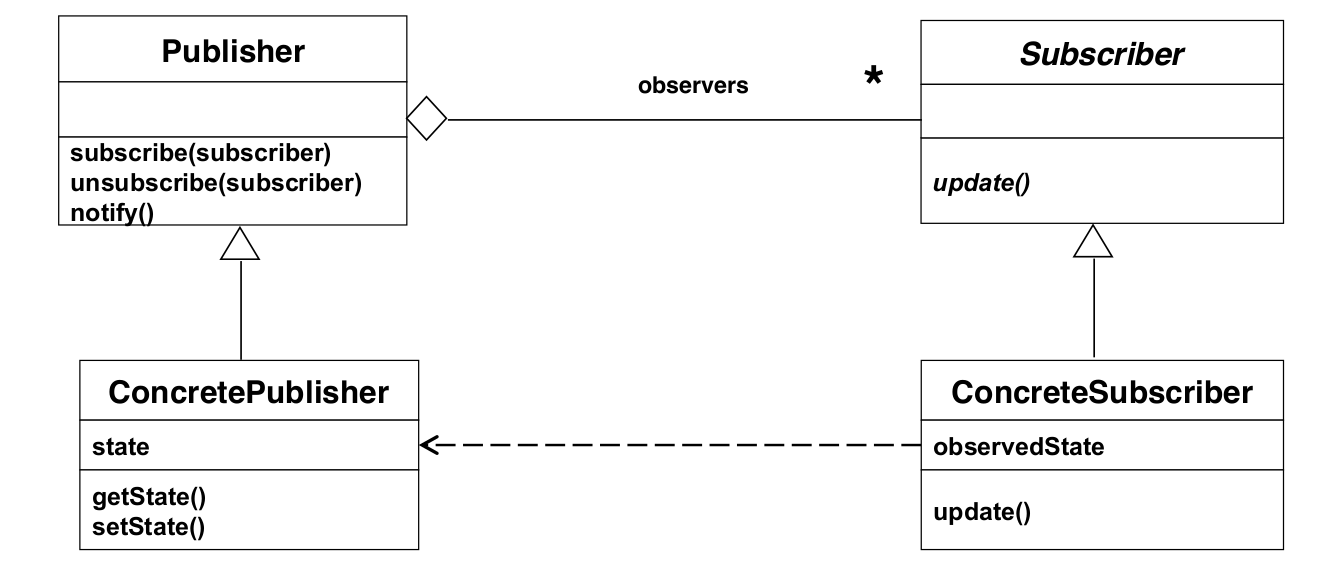
\includegraphics[width=\linewidth]{design_pattern/observer.png}

% \subsubsection{Model View Controller Pattern}
